\section{Selected observed results}
\label{sec:selected-observed-results}
% Generated from the frozen v4.9.12 result ledger; do not edit by hand.
\newcommand{\FinalSixteenSupportLowMeV}{30}
\newcommand{\FinalSixteenSupportHighMeV}{210}
\newcommand{\FinalSixteenLengthScaleUpperFactor}{12}
\newcommand{\SelectedAllThreeMinMass}{66}
\newcommand{\SelectedAllThreeMinP}{2.845\times 10^{-3}}
\newcommand{\SelectedAllThreeMinZ}{2.765}
\newcommand{\SelectedSharedEpsTwoHat}{4.550\times 10^{-6}}
\newcommand{\SelectedSharedEpsTwoSigma}{1.649\times 10^{-6}}


This is a snapshot of a partially unblinded analysis. It includes the fully unblinded
2015 and 2016 samples and the 10\% sample currently available from 2021. The
remaining 2021 data will be unblinded shortly, so the curves below describe the
observed result in hand rather than projecting the reach of the full 2021 sample.

Each mass point uses the corrected, bounded, piecewise-asymptotic \CLs{}
construction with the common signal-strength coordinate constrained to
$\eps^2\geq 0$. The Gaussian-process supports, hyperparameter states, and physics
normalizations are frozen before the observed limits and $p_0$ values are evaluated.
The inference is conditional on those frozen choices and on
the asymptotic approximation. For 2016, the frozen GP support is
\FinalSixteenSupportLowMeV--\FinalSixteenSupportHighMeV~MeV and the upper
resolution-scaled length-scale factor is \FinalSixteenLengthScaleUpperFactor. The
2015 and 2021 configurations retain their separately qualified supports.
One numerical caveat applies to 2016. An independent cross-process replay passed the
specified $10^{-6}$ state-reproduction check at 87 of 142 masses. A downstream replay
with the optimizer disabled, together with the other release checks, passes; even so,
every 2016-inclusive curve remains preliminary and conditional on this exception.

The three current inputs can be analyzed in seven distinct combinations: each data set
alone, each of the three pairs, and all three together.

\begin{center}
\small
\begin{tabularx}{\linewidth}{@{}P{0.15\linewidth}Y P{0.28\linewidth}@{}}
\toprule
Scope & Active data sets & Statistical coordinate \\
\midrule
Standalone & full 2015 & campaign-specific $\eps^2$ \\
Standalone & full 2016 & campaign-specific $\eps^2$ \\
Standalone & 2021 10\% & campaign-specific $\eps^2$ \\
Pair & full 2015 + full 2016 & one shared $\eps^2$ \\
Pair & full 2015 + 2021 10\% & one shared $\eps^2$ \\
Pair & full 2016 + 2021 10\% & one shared $\eps^2$ \\
All three & full 2015 + full 2016 + 2021 10\% & one shared $\eps^2$ \\
\bottomrule
\end{tabularx}
\end{center}

No expected-limit bands or toy-calibrated limit ensembles are included at this
stage. The background-only $p_0$ values are fixed-mass, one-sided asymptotic
quantities. They have no look-elsewhere correction and must not be interpreted as
global significances. Nor do they constitute a direct coverage calibration of the
upper-limit construction.

\subsection{Each data set on its own}
\label{sec:selected-individual-results}

Figure~\ref{fig:individual-final-results} shows one curve for each current input.
The likelihood is evaluated in the fitted window in event-count coordinates. The top
panel shows the full-template signal yield implied by the resulting observed 90\%
\CLs{} limit; the middle panel gives the same limit on $\eps^2$ after applying the
campaign-specific exposure, efficiency, resolution, radiative fraction, and
branching inputs; and the bottom panel gives the local asymptotic $p_0$. The two
limit views make the normalization convention explicit without treating the
full-template yield as a separately fitted quantity.

\begin{figure}[htbp]
  \centering
  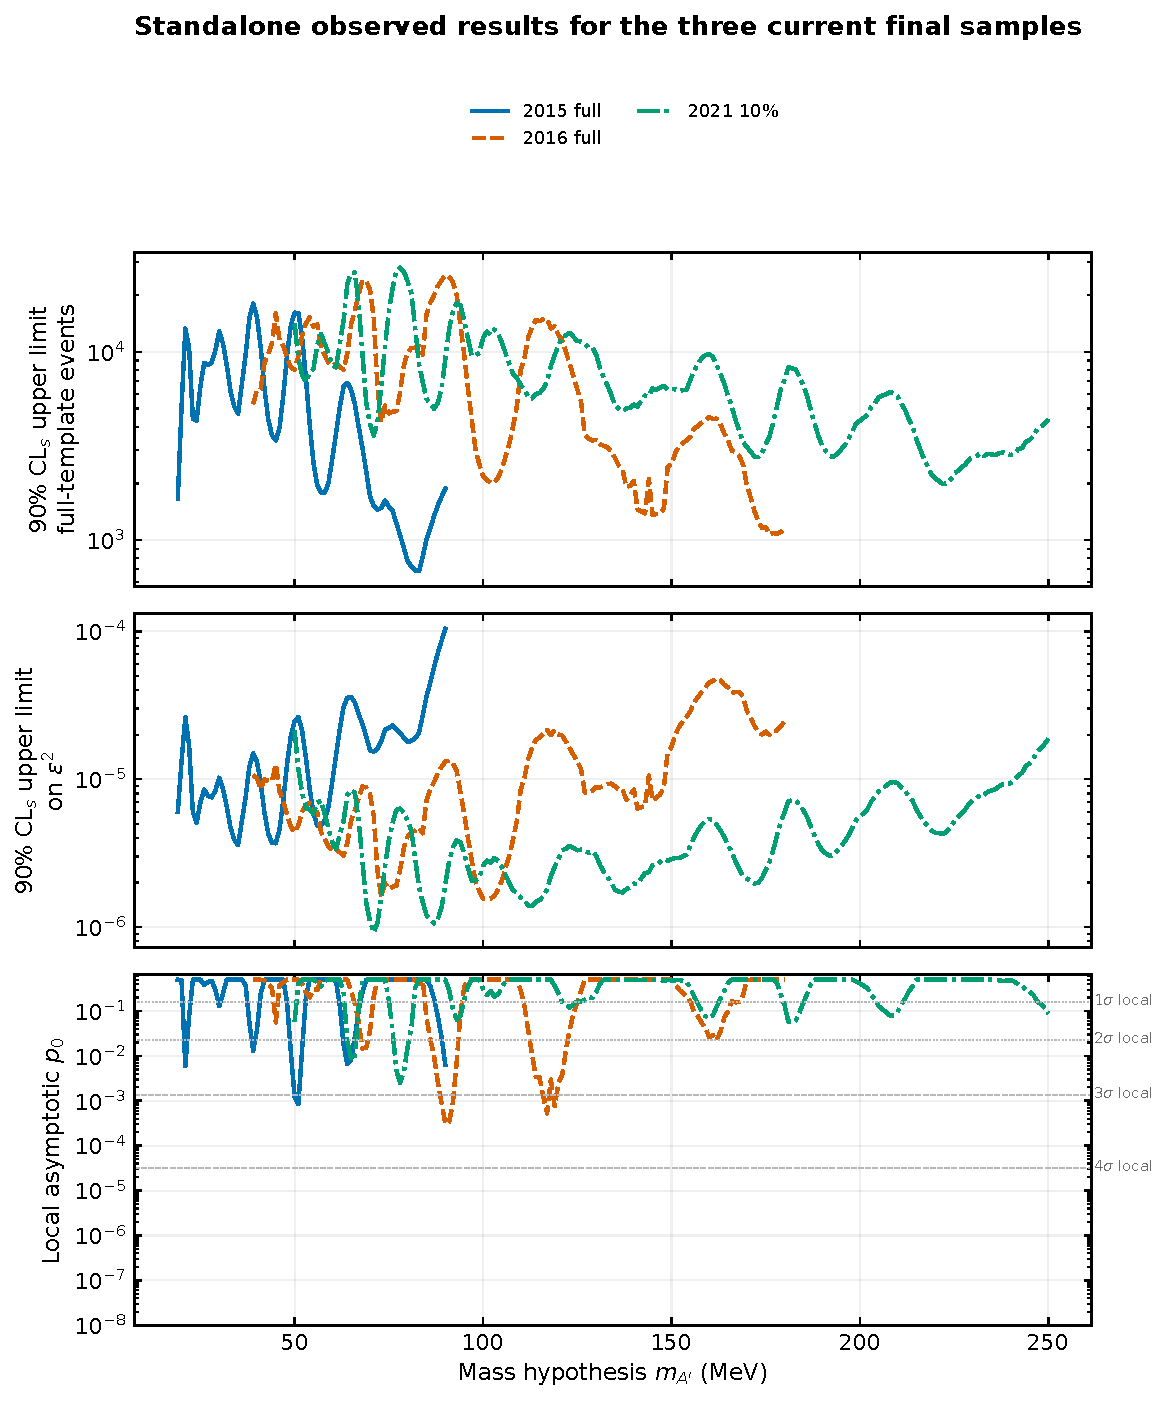
\includegraphics[width=0.98\linewidth]{../figures/individual_final_results.pdf}
  \caption{Observed standalone results for full 2015, full 2016, and the 2021
  10\% sample. From top to bottom, the panels show the 90\% bounded,
  piecewise-asymptotic \CLs{} signal-yield upper limit, the corresponding
  electron-channel $\eps^2$ upper limit, and the local asymptotic background-only
  $p_0$. The GP state is frozen independently for each campaign. No expected-limit
  bands are shown.}
  \label{fig:individual-final-results}
\end{figure}

The lower-exposure 2016 sample helped develop the 2016 support study, but it does not
appear as a fourth observed curve. Every combination below uses the full-2016 scan.

\FloatBarrier
\subsection{Combining data sets through a shared coupling}
\label{sec:selected-combined-results}

Figure~\ref{fig:combined-final-results} contains all three pairwise combinations and
the all-three result. At any given mass, the simultaneous likelihood profiles one
nonnegative $\eps^2$ shared by the active campaigns. Each campaign nevertheless
retains its own signal normalization, GP prediction, covariance, and observed
spectrum. Combining the data sets is thus a new likelihood calculation, not an
envelope, average, or choice among the standalone limits. Each curve is evaluated only
on the mass interval common to all of its active inputs.

\begin{figure}[htbp]
  \centering
  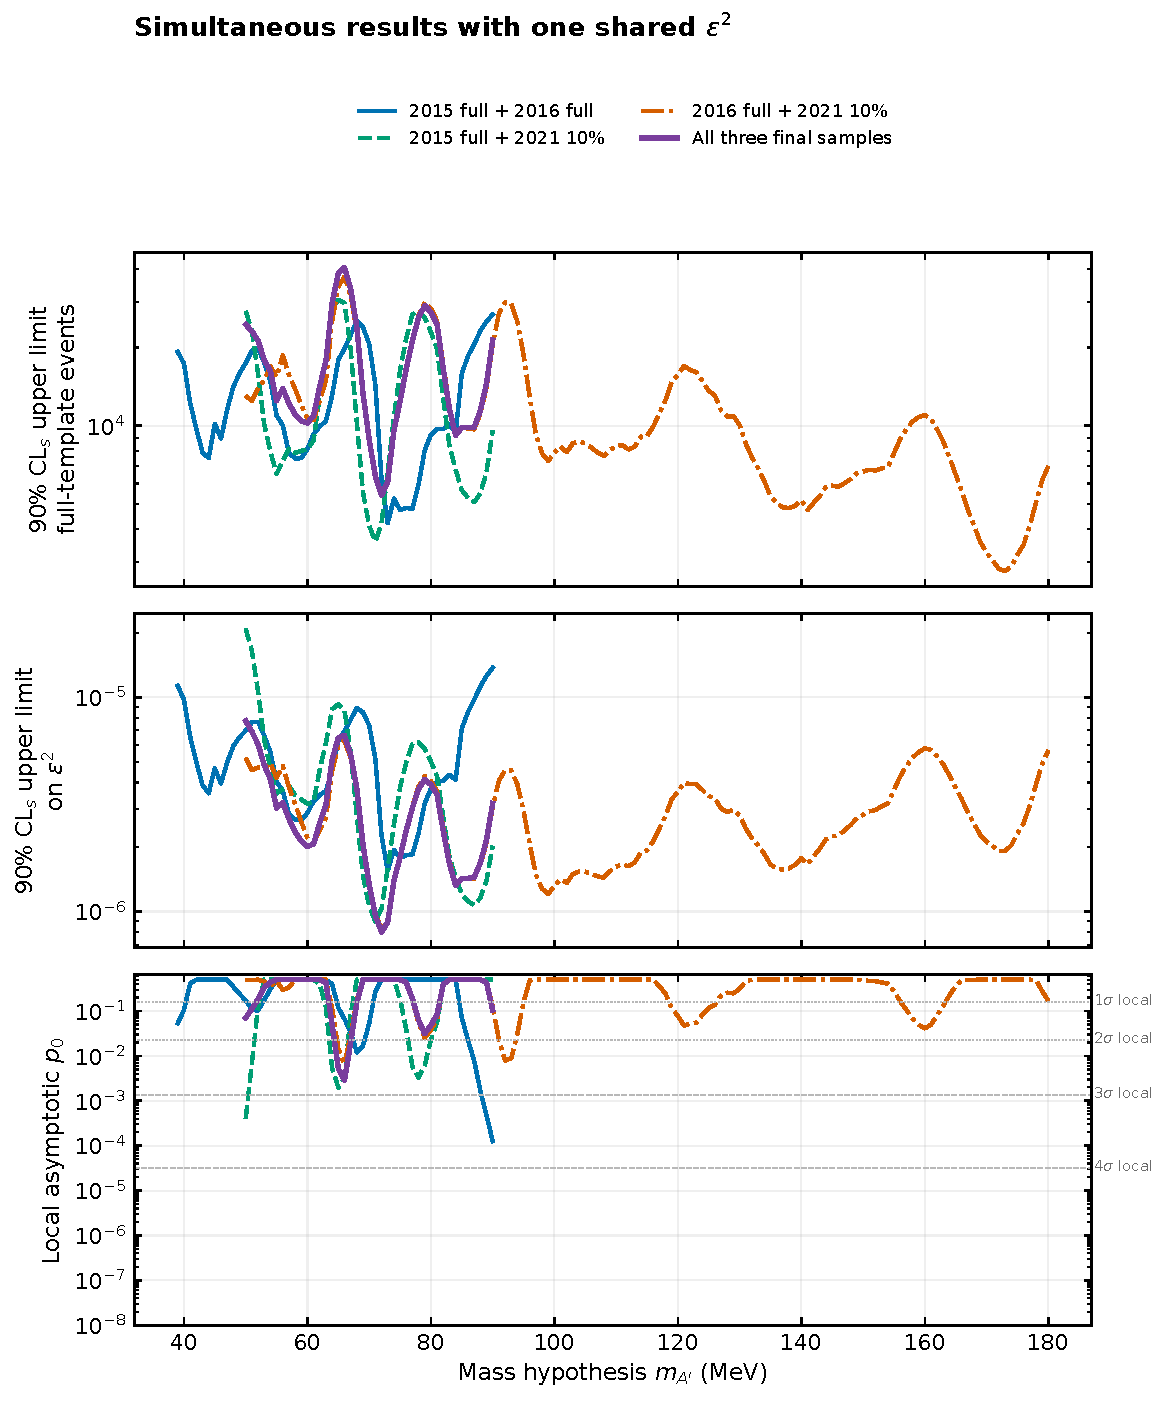
\includegraphics[width=0.94\linewidth]{../figures/combined_final_results.pdf}
  \caption{Observed shared-$\eps^2$ results for the three pairwise combinations
  and the all-three overlap. For visual alignment, the top coordinate expresses the
  shared-coupling limit as the total compatible signal yield summed over the active
  campaigns. The middle panel gives the 90\% bounded, piecewise-asymptotic \CLs{}
  upper limit on $\eps^2$, and the bottom panel gives the local asymptotic $p_0$.
  No expected-limit bands are shown.}
  \label{fig:combined-final-results}
\end{figure}

The shared coupling expresses the physical relationship among the campaigns: a
putative dark photon has one $\eps^2$, while its expected event count
changes with beam conditions, exposure, acceptance, and mass resolution. It also
keeps the independent background information from each spectrum explicit.

\FloatBarrier
\subsection{Local asymptotic scans}
\label{sec:selected-local-p0-series}

Figure~\ref{fig:final-asymptotic-pvalues} places the local $p_0$ scans for all seven
cases on the same axes, making structure at a common mass easier to compare across
campaigns. Every plotted point is still a separate fixed-mass test. Without a
scan-wide background-only calibration, none of these curves supports a statement
about global significance.

\begin{figure}[htbp]
  \centering
  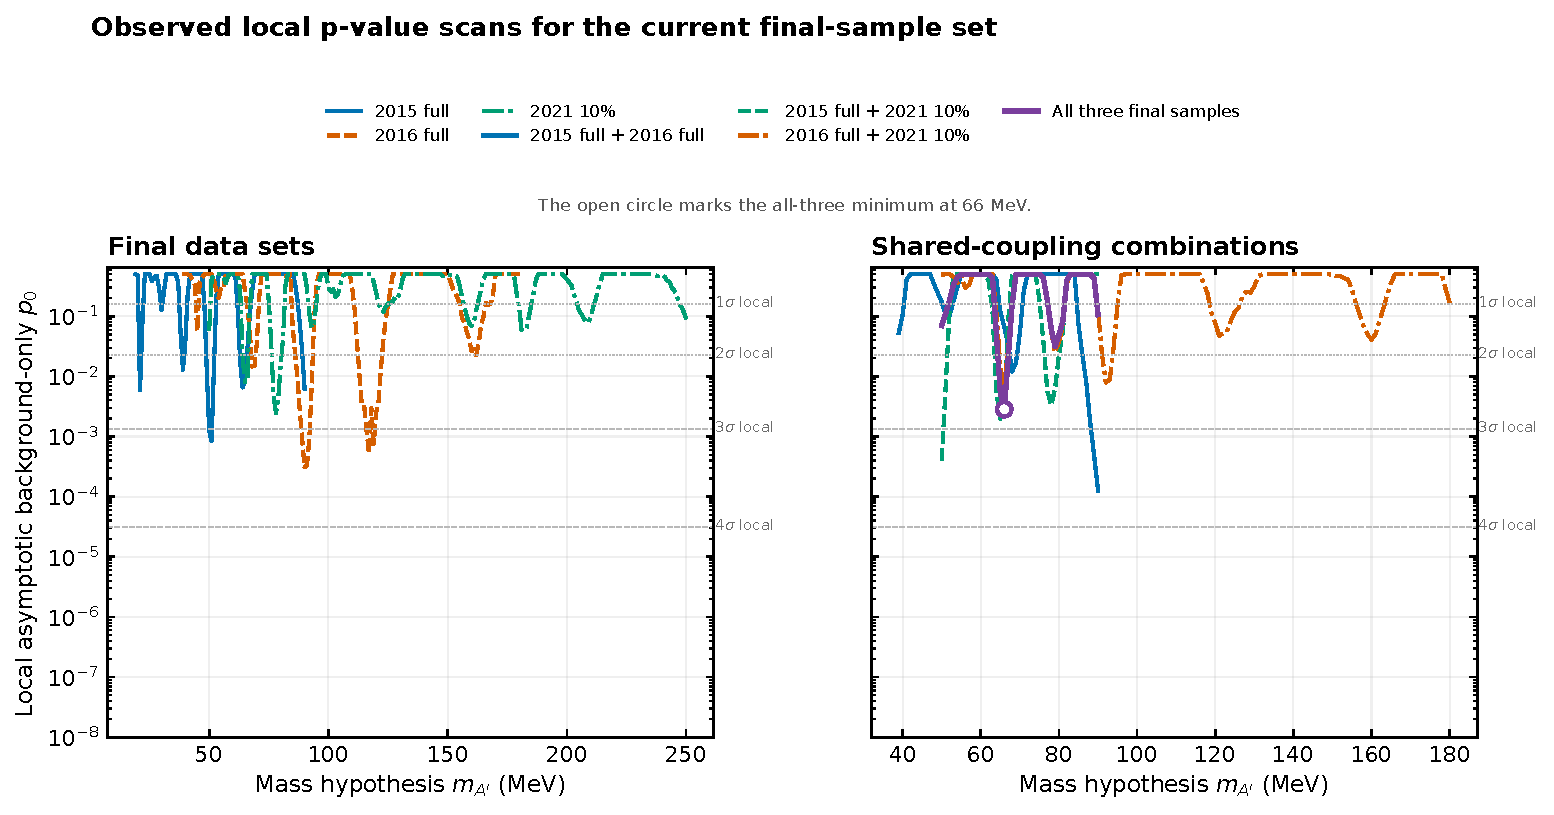
\includegraphics[width=0.98\linewidth]{../figures/final_asymptotic_pvalues.pdf}
  \caption{Local one-sided asymptotic background-only $p_0$ for the three
  standalone inputs, the three pairs, and the all-three combination. The values are
  conditional on the frozen GP supports and states. No look-elsewhere correction,
  global significance, or toy calibration is reported.}
  \label{fig:final-asymptotic-pvalues}
\end{figure}

\FloatBarrier
\subsection{Extraction at the largest all-three local fluctuation}
\label{sec:selected-all-three-extraction}

Within the common three-campaign interval, the smallest local asymptotic value occurs
at \SelectedAllThreeMinMass~MeV, where
$p_0=\SelectedAllThreeMinP$ and
$Z=\SelectedAllThreeMinZ$ under the one-sided local asymptotic mapping.
The corresponding shared fit is
$\widehat{\eps^2}=\SelectedSharedEpsTwoHat\pm\SelectedSharedEpsTwoSigma$.
Figure~\ref{fig:all-three-peak-extraction} decomposes the corresponding shared-signal
fit into the three statistically independent spectra. Showing the data, frozen GP
background prediction, and fitted signal contribution together makes clear which
campaigns support or constrain the common-coupling fluctuation.

\begin{figure}[htbp]
  \centering
  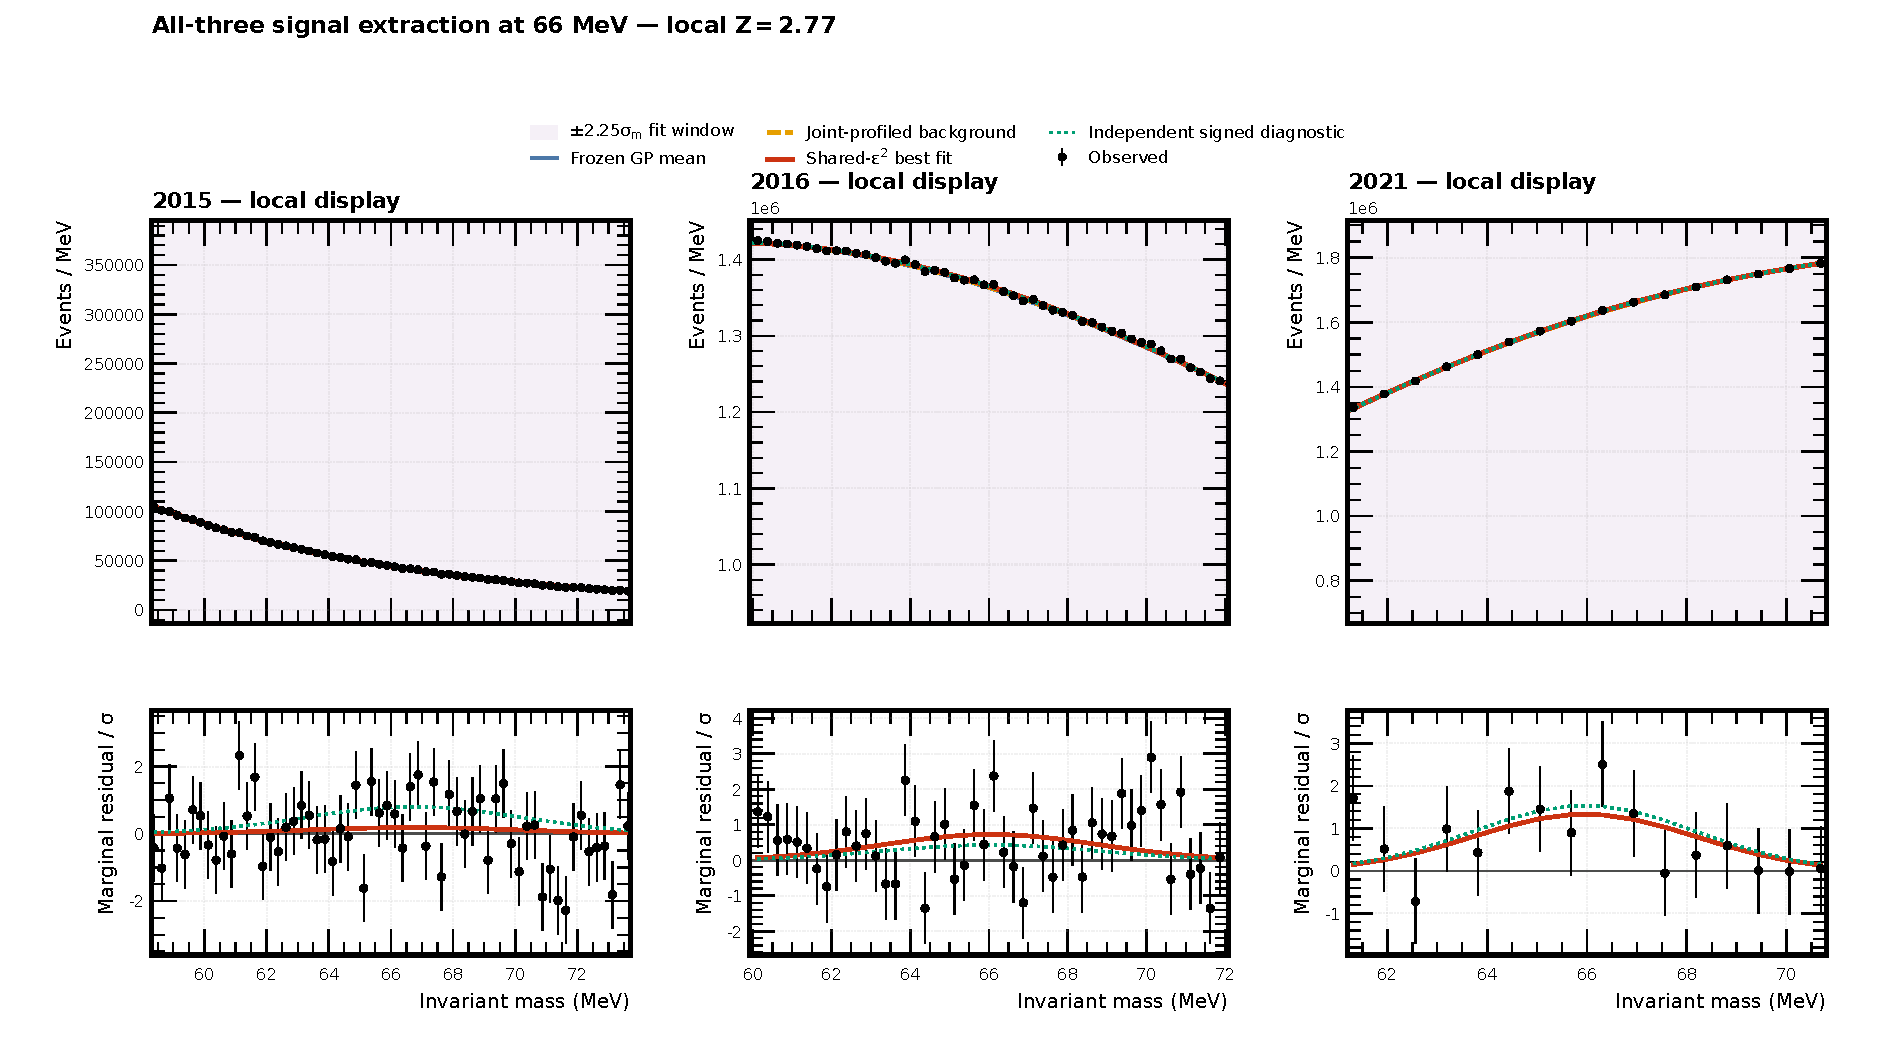
\includegraphics[width=0.98\linewidth]{../figures/all_three_peak_extraction.pdf}
  \caption{Signal extraction at \SelectedAllThreeMinMass~MeV, the mass hypothesis
  with the smallest local asymptotic $p_0$ in the all-three scan. The panels show
  full 2015, full 2016, and the 2021 10\% sample with their frozen GP background
  descriptions and the signal contribution from the shared-$\eps^2$ profile fit.
  The quoted $p_0$ and $Z$ are local asymptotic diagnostics, not a scan-calibrated
  discovery claim.}
  \label{fig:all-three-peak-extraction}
\end{figure}

\FloatBarrier
% Generated from all_three_peak_extraction_table.csv; do not edit by hand.
\begin{table}[htbp]
  \centering
  \small
  \begin{tabular}{@{}lrrr@{}}
  \toprule
  Data set & Shared full yield & Shared window yield & Independent signed window yield \\
  \midrule
  2015 & $725.51 \pm 262.85$ & $708.49 \pm 256.68$ & $3074.70 \pm 1588.39$ \\\\
  2016 & $12250.64 \pm 4438.30$ & $11927.18 \pm 4321.11$ & $7057.48 \pm 6658.90$ \\\\
  2021 & $14866.70 \pm 5386.08$ & $14584.36 \pm 5283.78$ & $16816.92 \pm 7106.66$ \\\\
  \bottomrule
  \end{tabular}
  \caption{Signal-yield decomposition at the all-three local-$p_0$ minimum. The shared columns use one common $\epsilon^2$. The signed campaign-level fits are post-selection concordance diagnostics, not independent measurements.}
  \label{tab:all-three-peak-extraction}
\end{table}


\FloatBarrier
